\section{Introduzione}

TODO: rivdere questa introduzione (io la rivedrei)

Data la straordinarietà degli eventi che erano in corso dal punto di vista sanitario nel nostro paese si è reso necessario svolgere gran parte del lavoro in modalità a distanza e quindi senza la possibilità di testare il modello matematico appena ottenuto e i successivi risultati dovuti all'azione di controllo sul V.A.B., il lavoro quindi è stato svolto per la maggior parte sfruttando il tool \textit{Simulink} di Matlab che è, in poche parole, un risolutore di equazioni differenziali.

Abbiamo così adottato una metodologia di lavoro basata su prototipi sempre più simili a quello che dovrebbe essere il sistema reale.

Si va ora ad analizzare la risposta del sistema al controllo ottenuto nei punti precedenti, per assicurarci, che quanto scritto sopra valga oltre che nella teoria anche nella pratica:
\begin{figure}[H]
	\centering   	
	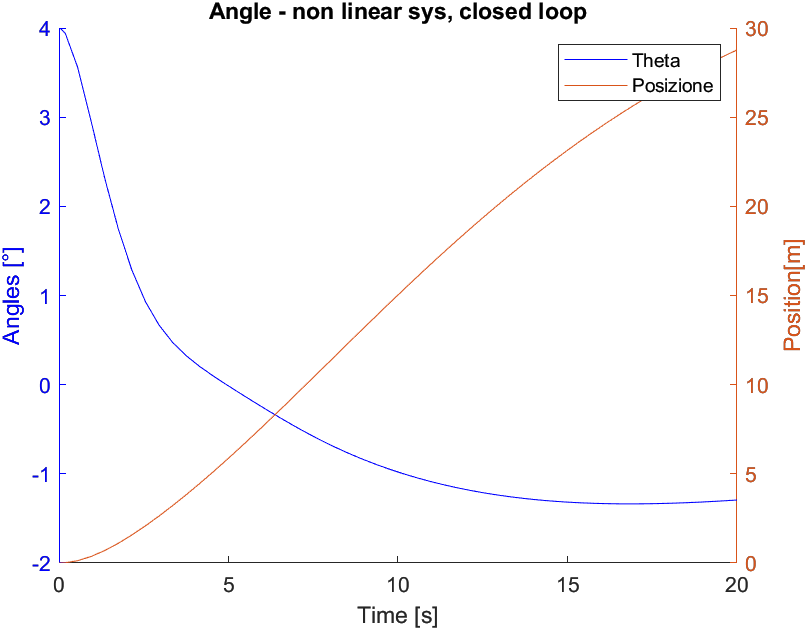
\includegraphics[width=0.7\textwidth]{Immagini/closed_loop_non_linear.png}
	\caption{Risposta del sistema non lineare in anello chiuso}
	\label{fig:closed_loop_non_linear_response}
\end{figure}
\begin{figure}[H]
	\centering   	
	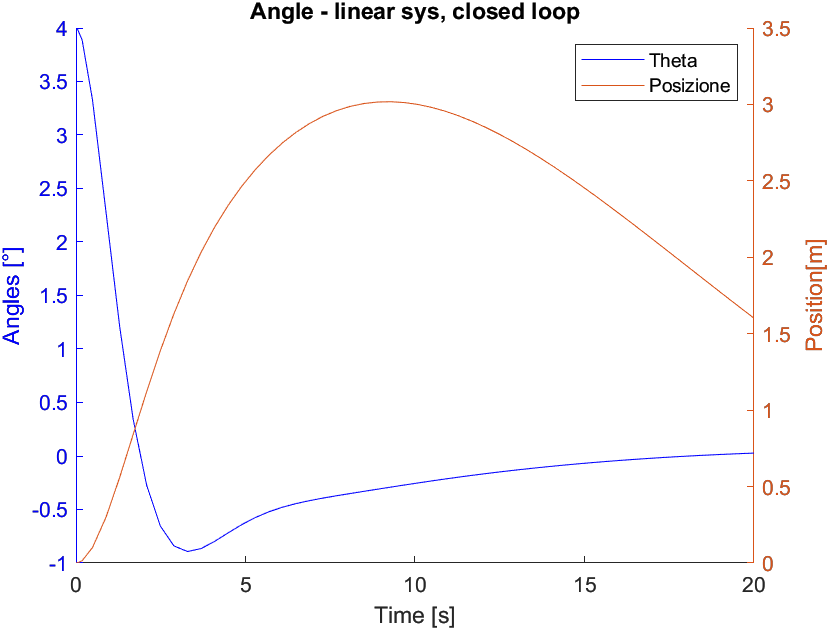
\includegraphics[width=0.7\textwidth]{Immagini/closed_loop_linear.png}
	\caption{Risposta del sistema lineare in anello chiuso}
	\label{fig:closed_loop_linear_response}
\end{figure}
TODO: come spieghiamo la differenza? rifare la simulazione?



\section{Simulazione del sistema non lineare}

Il primo compito che abbiamo risolto è stato quello di implementare le equazioni differenziali ottenute nel capitolo precedente:
\begin{itemize}
	\item $\ddot{\phi} = f_{\ddot{\phi}} (M_c,\theta,\dot{\theta},C_m)$
	\item $\ddot{\theta} = f_{\ddot{\theta}} (M_c,\theta,\dot{\theta},C_m)$
\end{itemize}

Dove $M_c$ sarebbe la massa del passeggero, $\theta e \dot{\theta}$ lo stato del sistema e $C_m$  la coppia erogata dal motore. Si può notare come entrambe le equazioni differenziali siano indipendenti dalla coordinata libera $\phi$.
\begin{figure}[H]
	\centering   	
	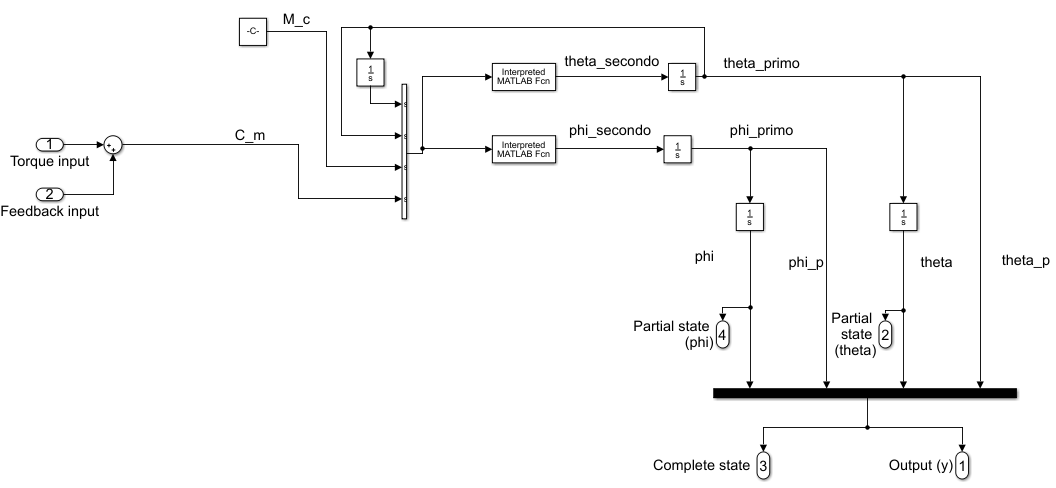
\includegraphics[width=1\textwidth]{Immagini/non_linear_system.png}
	\caption{Implementazione simulink delle equazioni differenziali}
	\label{fig:non_linear_system}
\end{figure}
In Fig.\ref{fig:non_linear_system} le \textit{interpreted function} altro non sono che  $f_{\ddot{\phi}}$ e $f_{\ddot{\theta}}$. A valle di esse sono presenti degli integratori che permettono di ottenere lo stato $x$ completo del sistema. Si può facilmente notare come $\dot{\theta} e \theta$ siano collegate direttamente all'input delle \textit{interpreted function}.
Si è dunque proceduto a  simulare il sistema per verificare la bontà di quanto ottenuto; in particolare, il sistema in anello aperto, dovrebbe oscillare all'infinito vista la mancanza di attriti nel modello.

\begin{figure}[H]
	\centering   	
	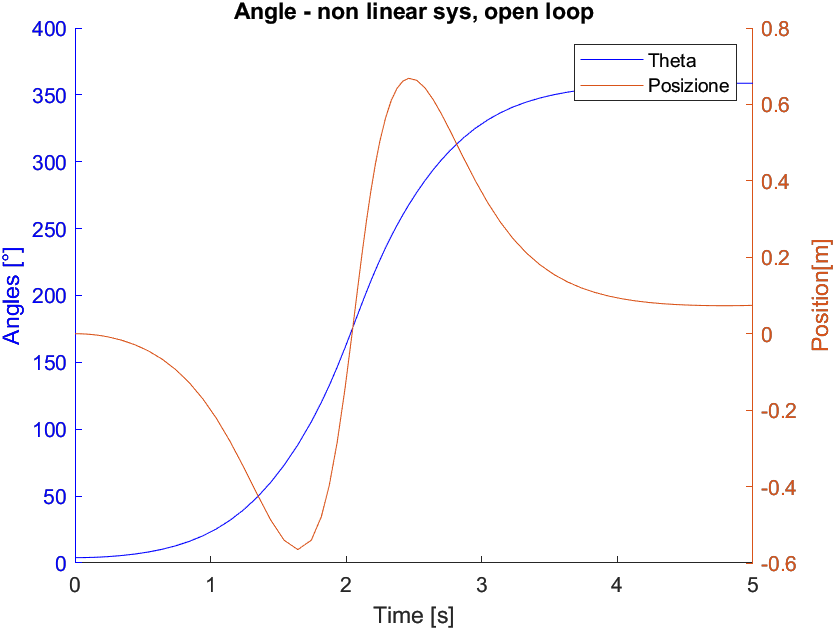
\includegraphics[width=0.6\textwidth]{Immagini/open_loop_response_non_linear.png}
	\caption{Risposta in anello aperto del sistema reale}
	\label{fig:open_loop_response_non_linear}
\end{figure}
La simulazione, il cui risultato è riportato in Fig.\ref{fig:open_loop_response_non_linear} è stata svolta per 5 secondi e con un angolo iniziale di 4°; il grafico mostra dunque l'andamento di $\theta$ nel tempo e della posizione che in termini matematici si esprime come $posizione = \phi \cdot{r_{ruota}}$
\label{sec:simulazione_reale}
\section{Simulazione del sistema lineare}
Si è inoltre creato un altro modello sfruttando il sistema lineare ottenuto prima  con l'obbiettivo di semplificare il problema e di velocizzare le simulazioni con lo scopo di testare rapidamente nuove tecniche di controllo che se avessero dato esito positivo sul modello lineare sarebbero poi state testate sul simulink che imita il comportamento reale del sistema.
\begin{figure}[H]
	\centering   	
	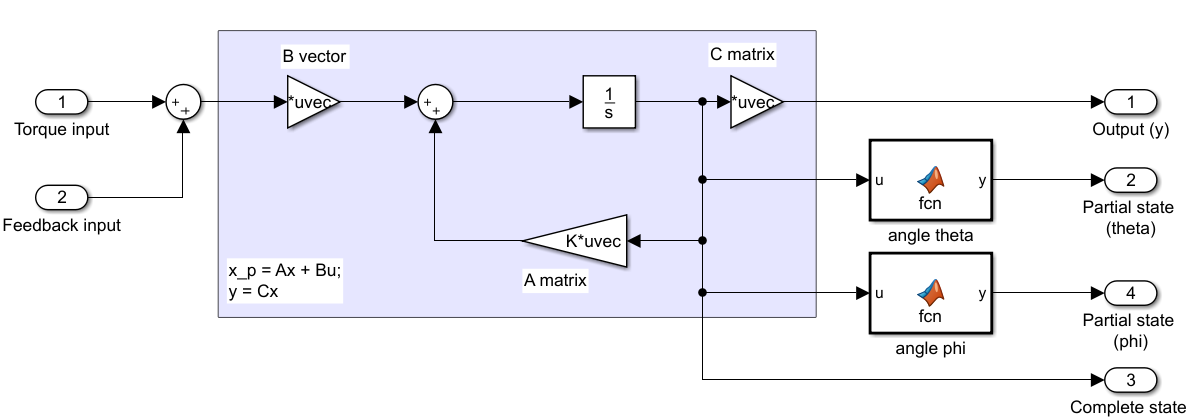
\includegraphics[width=1\textwidth]{Immagini/linear_system.png}
	\caption{Implementazione simulink del sistema linearizzato}
	\label{fig:linear_system}
\end{figure}

\begin{figure}[H]
	\centering   	
	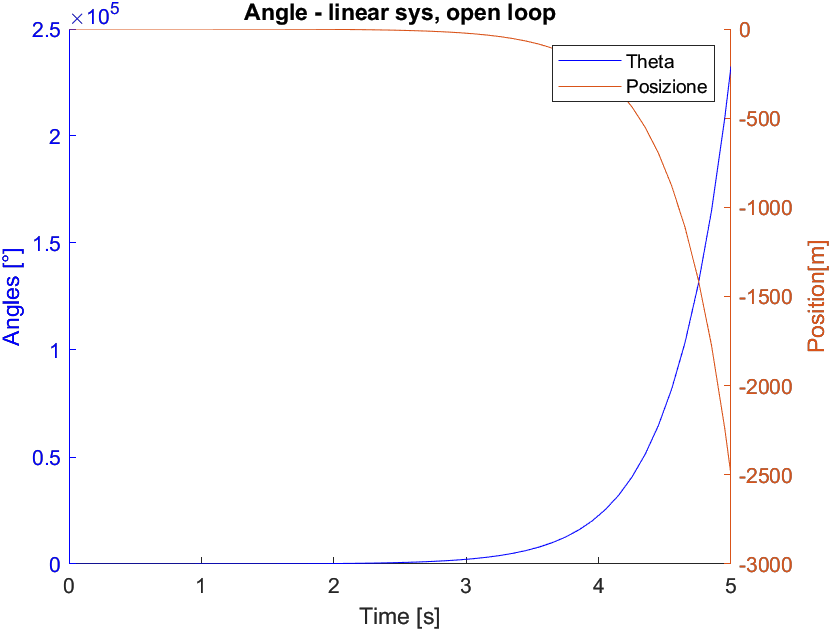
\includegraphics[width=0.6\textwidth]{Immagini/linear_open_loop.png}
	\caption{Risposta in anello aperto del sistema lineare}
	\label{fig:open_loop_response}
\end{figure}
In questo caso, la simulazione in anello aperto mostra che il sistema diverge; questo perché la linearizzazione ha senso attorno al punto di equilibrio da cui è stata ottenuta, distante da quel punto il sistema lineare non approssima più il sistema reale ed anche un eventuale controllo ottenuto da esso non garantisce buone performance distante da quel punto. Si nota, in Fig.\ref{fig:open_loop_response} che il punto di partenza è 4° e il sistema, lineare, diverga quasi immediatamente; la differenza con la risposta del sistema non lineare in Fig.\ref{fig:open_loop_response_non_linear}

Come già verificato in precedenza (sezione ~\ref{sec:open_loop_analysis}) ci sono due poli reali, uno negativo e uno positivo; questo dimostra come il sistema sia instabile in anello aperto e necessiti di controllo.

\section{Motore}
Il passo successivo è stato quello di andare a modellizzare il motore presente a bordo dello chassis; questo è necessario in quanto si deve tenere conto, in primo luogo, del ritardo che gli attuatori ( cioè il motore) introducono nel sistema e che per questo potrebbe diventare instabile.
\begin{figure}[H]
	\centering   	
	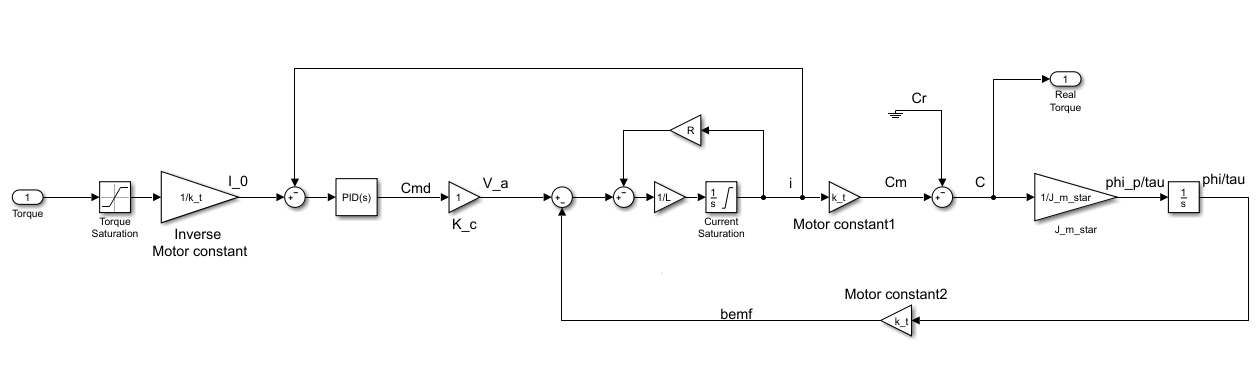
\includegraphics[width=1\textwidth]{Immagini/motor.png}
	\caption{Schema a blocchi del motore}
	\label{fig:motor}
\end{figure}

I valori delle componenti in Fig.\ref{fig:motor} sono presi dal datasheet del motore.
Il controllo del motore DC in questione e stato ottenuto tramite una retroazione in corrente che permette quindi di definire un setpoint alla corrente presente nel motore. Questo si è reso necessario poiché il controllore, attraverso il vettore K e lo stato del sistema, definisce la coppia che il motore dovrebbe erogare. In un motore DC la correlazione tra coppia erogata e corrente esiste ed è ben definita e si tratta di $k_t$.
Il controllore è stato realizzato seguendo metodi già noti in letteratura TODO: scrivere la formula o trovare un posto che la spieghi 
\begin{figure}[H]
	\centering   	
	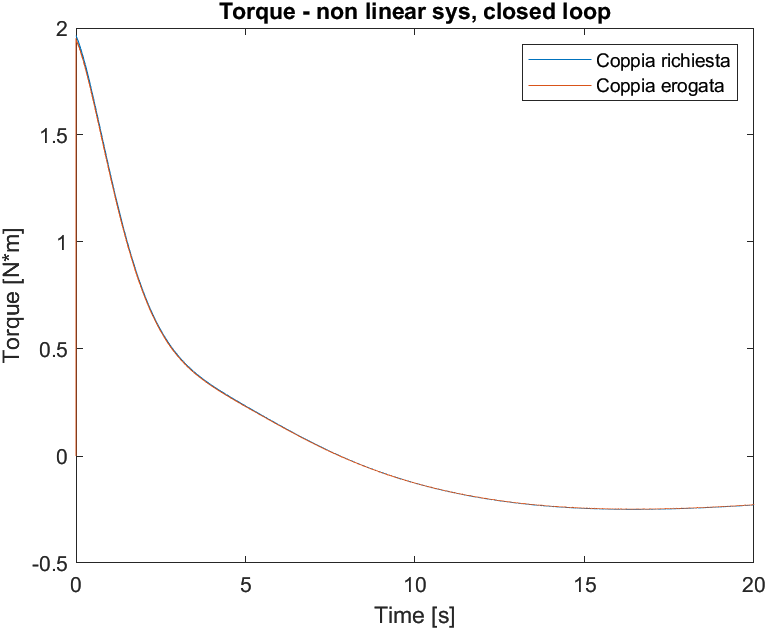
\includegraphics[width=0.7\textwidth]{Immagini/motore.png}
	\caption{Transitorio del motore}
	\label{fig:motore}
\end{figure}
\begin{figure}[H]
	\centering   	
	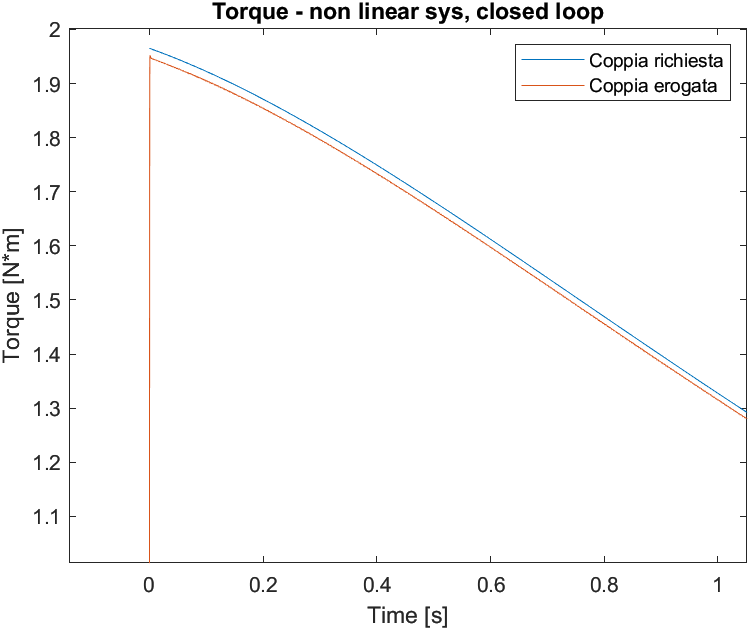
\includegraphics[width=0.7\textwidth]{Immagini/motore_zoom.png}
	\caption{Zoom del grafico in figura Fig.\ref{fig:motore}}
	\label{fig:motore_zoom}
\end{figure}

Come si può notare il picco di coppia massimo è minore di 2; questo è dovuto al fatto che, per ragioni esterne, nel motore può scorrere ua corrente di massimo 20A e quindi:
\begin{center}
	$C_{m,max} = I_{max}\cdot{K_{motore}} = 20 A\cdot{10 \dfrac{N\cdot{m}}{A}}=2N\cdot{m}$
\end{center}

Un esempio in cui la coppia richiesta supera i $2N\cdot{m}$ è il seguente:
\begin{figure}[H]
	\centering   	
	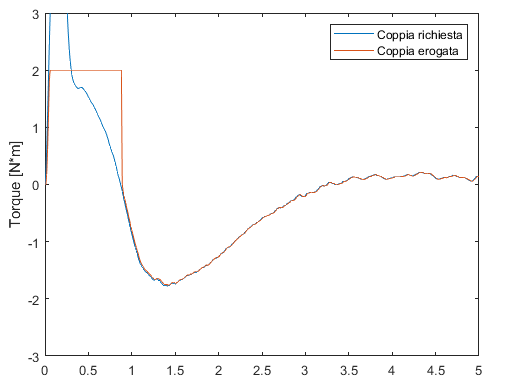
\includegraphics[width=0.8\textwidth]{Immagini/saturazione.png}
	\caption{Clamp della coppia erogata da parte del motore}
	\label{fig:clamp_motore}
\end{figure}
In Fig.\ref{fig:clamp_motore} è anche possibile notare come l'assenza del blocchetto denominato \textit{Torque saturation}, presente in Fig.\ref{fig:motor}, satura l'azione integrale dell'attuatore e inserisce un ritardo non secondario nell'azione di controllo.
\section{Modello complessivo (al momento)}
L'obbiettivo di questo paragrafo è quello di fare il punto della situazione del sistema sviluppato fino a questo punto e di sviluppare alcune considerazioni sul lavoro fatto.

\begin{figure}[H]
	\centering   	
	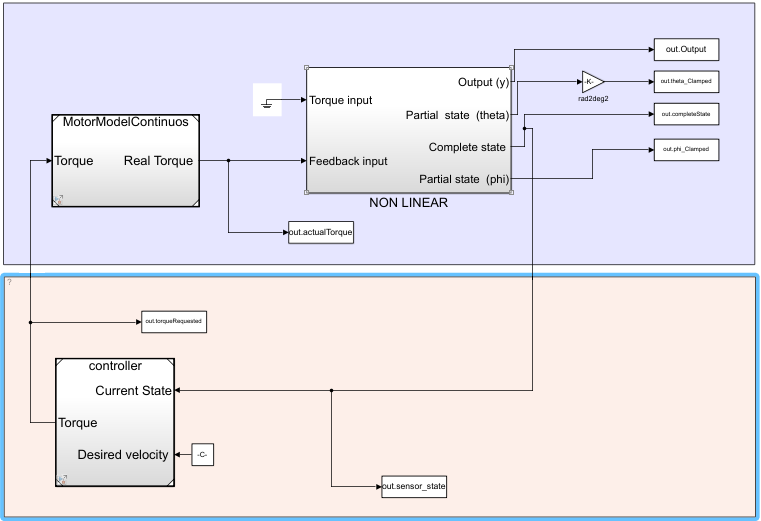
\includegraphics[width=0.8\textwidth]{Immagini/simulink_model_continuos.png}
	\caption{Simulink}
	\label{fig:simulink}
\end{figure}
Come si osserva in Fig.\ref{fig:simulink} il sistema al momento comprende tre blocchi:
\begin{itemize}
	\item Il blocco \textit{non linear}: rappresenta quello che nella realtà sarebbe il sistema reale; si occupa durante la simulazione, dati gli input, di restituire output simili a quelli che si avrebbero in laboratorio utilizzando la macchina vera e propria.
	\item Il blocco \textit{MotorModelContinuos}: si occupa di simulare la presenza e i transitori dovuti ai motori che nella realtà sono posti a bordo dello chassis.
	\item Il blocco \textit{controller}: è, dei tre, l'unico blocco che effettivamente dovrebbe essere implementato su un calcolatore. Con i valori simulati dai due blocchi di cui sopra calcola il valore di coppia per il controllo e lo fornisce indietro ai suddetti blocchi per completare la retroazione.
\end{itemize}
Il sistema al momento è, in linea teorica, a tempo continuo. Nella realtà in un computer e in particolar modo su Simulink la possibilità di far operare i blocchi che simulano il sistema reale a tempo continuo è preclusa.
Si é scelto dunque,per quanto fatto finora, di lasciare scegliere al software di Simulink il passo della simulazione ed in particolar modo utilizzare un passo variabile. Questo permette, nei punti in cui le variazioni sono spiccate(ad esempio quando il sistema si avvia) di utilizzare un passo di simulazione anche dell'ordine dei nanosecondi che approssima quasi perfettamente l'esecuzione a tempo continuo.

\section{Discretizzazione}
Come già detto sopra, il controllore è necessario che sia implementato su u calcolatore e quindi verrà eseguito a tempo discreto; per tenere conto di questa caratteristica è necessario discretizzare il controllore e acquisire gli input a tempo discreto:
\begin{itemize}
	\item all'ingresso del blocco \textit{controller} è stato posto un \textit{Sample \& Holder}; questo blocco si occupa di acquisire ogni tempo di sampling $T_s$ il valore in input e mantenerlo inalterato fino alla lettura successiva
	\item all'uscita del \textit{controller} si è posizionato un altro \textit{Sample \& Holder} per le stesse ragioni
	\item il \textit{controller} è stato trasformato a tempo discreto; TODO inseriamo la cosa dei poli discreti o diciamo che sono uguali essendo un proporzionale?
	A differenza del controllore della retroazione dello stato, il controllore che chiude la retroazione in velocità va ricalcolato tenendo conto del $T_s$; fortunatamente Simulink fa da solo questa conversione se si setta il blocco simulink \textit{Controllore PID} come integratore a tempo discreto fornendo il $T_s$ e la costante moltiplicativa.
\end{itemize}
Il controllore a tempo discreto ha dunque questo aspetto nel modello simulink implementato:
\begin{figure}[H]
	\centering   	
	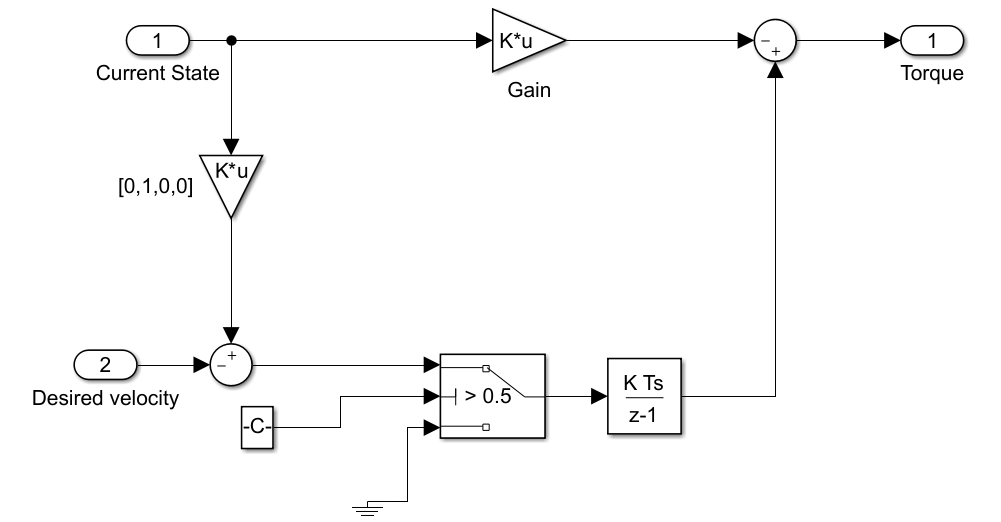
\includegraphics[width=0.8\textwidth]{Immagini/controller_discrete.png}
	\caption{Modello Simulink del controllore}
	\label{fig:controller_discrete}
\end{figure}

Per le stesse ragioni pratiche anche il modello del motore ha subito una conversione: il controllore dell'anello di retroazione in corrente sarà un software eseguito ciclicamente su di un calcolatore e va dunque implementato a tempo discreto.
Ricordando che la funzione che la F.d.T. del controllore \textit{PI} a tempo continuo era:
$$\dfrac{0.001216 s + 0.9965}{0.00122 s}$$
e applicando il metodo di Tustin da tempo continuo a discreto con un $T_s = 0.001$ si ottinene che:
$$\dfrac{1.405 z - 0.5881}{z - 1}$$

\section{Sensori}
Sempre con l'obbiettivo di rendere la simulazione più raffinata e accurata possibile sono stati inseriti all'interno del file simulink anche dei modelli che simulano la presenza dei sensori. Questo è necessario ed importante poiché nella realtà non esiste un modello matematico che genera i dati che poi sono dati in pasto al controllore ma si devono invece usare dei sensori che danno una stima dello stato del sistema. Un sensore presenta due principali caratteristiche: 
\begin{itemize}
	\item Rumore: è stato modellizzato come un \textit{Band-Limited
		White Noise} con \textit{Noise power} = [0.00000001] e \textit{Sample time} = 0.001.
	\item Quantizzazione: la lettura dei dati da un sensore, oltre ad avvenire ad un intervallo di tempo minimo e regolare, mostra anche un errore dovuto alla limitata sensibilità del sensore stesso o dell' \textit{ADC} che effettua la lettura. Il blocco simulink \textit{Quantizer} ha l'esatto scopo di simulare questo comportamento presente nei sensori reali.
\end{itemize}
TODO come spiego che mi arriva in ingresso theta e phi e non le derivate?
Sul sistema sono presenti diversi sensori:
\begin{itemize}
	\item Encoder incrementale: si occupa di misurare la rotazione della singola ruota
	\item I.M.U. : stima l'inclinazione dello chassis
	\item Sensore di corrente: misura la corrente presente nel motore
\end{itemize}
Per come si presenta il sistema, sia l'\textit{encoder} incrementale sia la \textit{I.M.U.} restituiscono rispettivamente una stima di $\phi$ e $\theta$
Per modellizzare quanto detto finora riguardante i sensori ed in particolare per l'\textit{encoder} e l'\textit{I.M.U.} è stato approntato il seguente blocco simulink:
\begin{figure}[H]
	\centering   	
	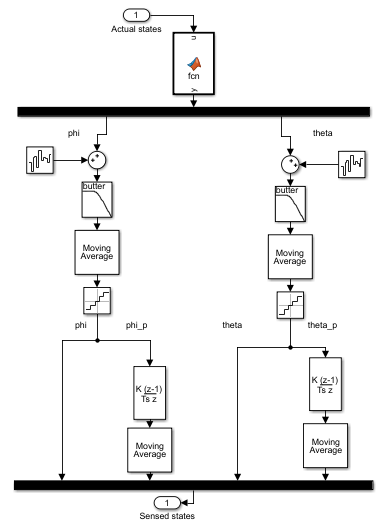
\includegraphics[width=0.8\textwidth]{Immagini/sensor_block1.png}
	\caption{Modello Simulink dei sensori \textit{encoder} e \textit{I.M.U.}}
	\label{fig:sensor_block1}
\end{figure}
Si può notare come in Fig.\ref{fig:sensor_block1} siano presenti due blocchi \textit{Moving average} per ciascun sensore; questo si è reso necessario per due ragioni.
La prima è che, presentando il sistema del rumore, era necessario rimuoverlo attraverso un filtro digitale; la seconda ragione è che, vista la presenza della quantizzazione, la derivazione a tempo discreto del segnale presenta molti picchi e molti valori nulli; è quindi necessario filtrare questi valori prima di passarli al controllore per evitare picchi di coppie troppo alti oppure nulli in brevi intervalli di tempo.
Si presenta ora la necessità di modellizzare la presenza del sensore di corrente nel motore; per fare ciò si è modificato solamente l'anello di retroazione esterno che permette il controllo del motore in corrente:

\begin{figure}[H]
	\centering   	
	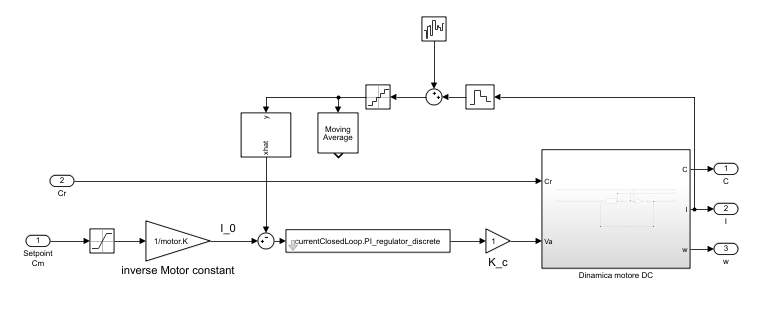
\includegraphics[width=0.8\textwidth]{Immagini/discrete_motor.png}
	\caption{Modello Simulink discreto del motore}
	\label{fig:discrete_motor}
\end{figure}
Si può notare in Fig.\ref{fig:discrete_motor} che il controllore è quello discreto presentato prima, mentre è stato inserito anche in questo caso un rumore sulla misura, una quantizzazione e un filtro sul segnale da passare al controllore.
Da sottolineare che ognuno dei tre blocchi \textit{Quantizer} ha un valore diverso dovuto al fatto che ognuno dei sensori ha sensibilità diverse:
\begin{itemize}
	\item Encoder incrementale: presenta una sensibilità di $2^11 bit = 2048 $ diverse combinazioni e letture
	\item I.M.U. : sensibilità del giroscopio di $131\dfrac{s}{deg}$
	\item Sensore di corrente: il valore del sensore di corrente è un voltaggio letto da un Arduino Uno con un ADC con sensibilità di 10 bit
\end{itemize}

\section{RTOS - XENOMAI}
Riportiamo di seguito una breve descrizione del lavoro portato avanti durante questa settimana per quanto concerne la parte RTOS.

\begin{itemize}
	\item Come prima cosa siamo andati a rivedere il file \textit{.cpp} che avevamo prodotto nelle settimane scorse. In particolare abbiamo dovuto ritoccare la parte relativa alla lettura dei dati dal file, andando ad utilizzare le API presenti in ambiente c invece di quelle relative a cpp.
	Abbiamo quindi provato e testato la lettura da file tramite il tool DevC++, facilitando così il testing e il debug;
	\item Siamo andati ad installare una macchina virtuale con installato a bordo \textbf{debian 9.8.0} e la patch \textbf{Xenomai 3.0.8} (\href{http://www.cs.ru.nl/lab/xenomai/}{link});
	\item Essendo debian un OS interamente fruibile da linea di comando, siamo andati a prendere confidenza con l'ambiente, andando a capire l'organizzazione e chiamando gli update/upgrade necessari;
	\item Prima di andare ad importare il file completo (di cui abbiamo parlato al punto iniziale), siamo andati ad eseguire alcuni esempi iniziali (una sorta di HelloWorld):
	\begin{itemize}
		\item Abbiamo per primo cosa studiato questo approccio iniziale (\href{http://www.cs.ru.nl/J.Hooman/DES/XenomaiExercises/Exercise-1.html}{link})
		\item Siamo andati ad impostare il funzionamento di un task (dummy) periodico, come se si trattasse appunto del main loop di Arduino (\href{http://www.cs.ru.nl/lab/xenomai/}{link})
	\end{itemize}
	
	\item Lo step successivo è stato quello di importare il codice scritto e testato in ambiente DevC++ in xenomai, provandolo e introducendo alcuni dettagli aggiuntivi:
	\begin{itemize}
		\item Periodo di funzionamento definito tramite questi comandi 
		\begin{lstlisting}
			RTIME period  = 1000000000; % Expressed in [ns]
			rt_task_set_periodic(NULL,TM_NOW,period);
		\end{lstlisting}
		\item Salvataggio dei parametri temporali now ad inizio del ciclo e update del parametro before alla fine del ciclo: questo per facilitare, in qualsiasi punto del codice, l'accesso ai parametri temporali per eventuali necessità di calcolo; inoltre abbiamo utilizzato questi parametri per definitire l'intervallo di tempo su cui andare a calcolare la derivata;
		\item Abbiamo seguito questo approccio nel ciclo principale eseguito a frequenza fissa: lettura file e sensori $\rightarrow$ algoritmo/elaborazione $\rightarrow$ produzione dei risultati di interesse;
		\item Il thread relativo al server opc - ua non è ancora stato gestito: esso sarà ovviamente lasciato in secondo piano rispetto al thread principale temporaizzato alla frequenza specifica;
	\end{itemize}
\end{itemize}
